Resolution studies characterize the precision of a timing reconstruction method but do not measure the accuracy of the reconstruction. It is possible to achieve a very precise result, and therefore an objectively good time resolution, by arbitrarily setting the reconstructed time of all rechits to a constant value with some random jitter. In order to test the accuracy of the reconstruction methods, the ability to compare the results of the reconstructed rechit time to a true time for that rechit is required. This is typically done with Monte-Carlo (MC) truth information. Unfortunately such information, while in development, is not available in current MC datasets.

\hfill
\begin{figure}[htbp]
\begin{center}
\resizebox{0.32\textwidth}{!}{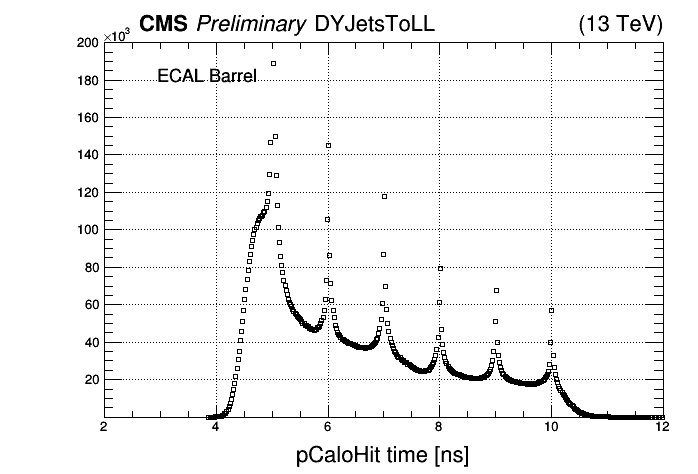
\includegraphics{fig/sec_gen/tr_pcalo_time_hit_18112020145605.png}}
\resizebox{0.32\textwidth}{!}{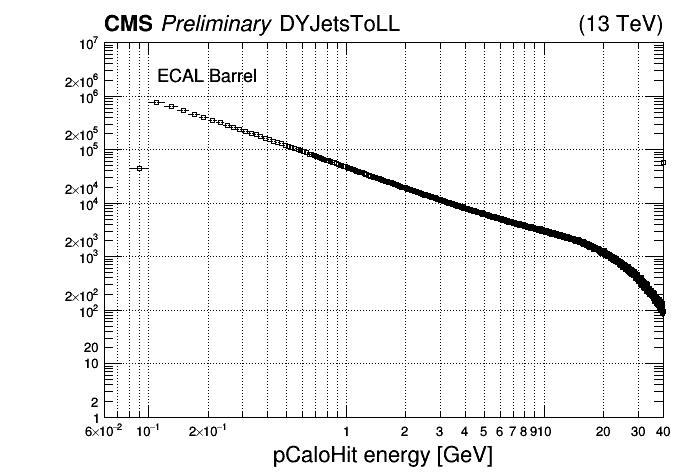
\includegraphics{fig/sec_gen/tr_pcalo_energy_hit_18112020150843.png}}
\resizebox{0.32\textwidth}{!}{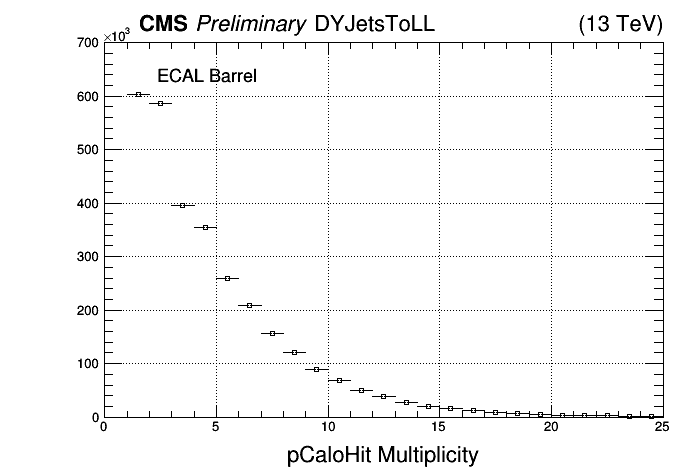
\includegraphics{fig/sec_gen/tr_pcalo_phomulti_hist_25112020111944.png}}
\caption{Time (left), energy (middle), and multiplicity (right) distributions of the pCaloHit information recorded in the pCaloHit collection.} 
\label{pc_etm}
\end{center}
\end{figure} 

In order to formulate a reference time, or \emph{gen time}, with existing MC that can be compared, rechit by rechit, with the reconstructed time, the information in the pCaloHit collection was utilized. The pCaloHit collection records the simulated deposition of energy in a crystal during an event and the time, relative to the bunch crossing, at which this energy was deposited in the crystal. Shower and event development may result in multiple energy depositions in a single crystal and at various depths within the crystal. A single pCaloHit is generated for each of the multiple energy depositions in a crystal. Unfortunately, while variables to record the depth information are present in the pCaloHit collection, in current simulation this information is not recorded by default. 

As can be seen in Figure~\ref{pc_etm} from the distributions of the time, energy, and multiplicity distributions of pCaloHit hits, the pCaloHit times are produced in smeared intervals from approximately five to ten nanoseconds, which is consistent with time of flight from the CMS origin to the physical location of the crystals. The pCaloHit times do not account for variations in the location of the interaction on the crystal face or the resolution of the location of the primary vertex. The energy and multiplicity distributions show that there are typically multiple pCaloHits in a crystal for any interaction and that these hits are produced with a uniform distribution of energy to be deposited in the crystals.

\hfill
\begin{figure}[htbp]
\begin{center}
\resizebox{0.7\textwidth}{!}{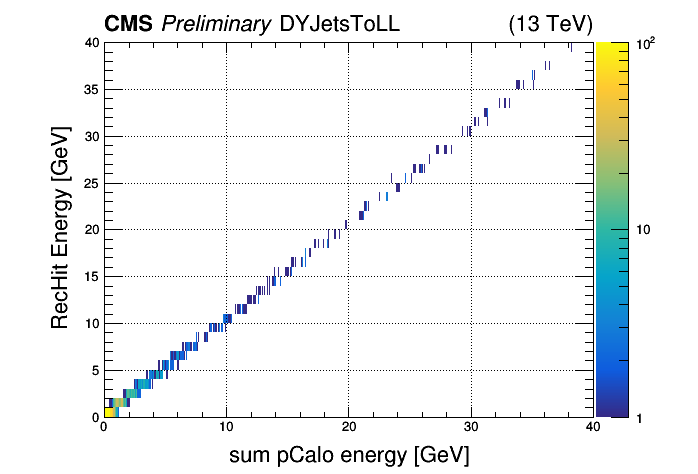
\includegraphics{fig/sec_gen/tr_2d_pce_v_rhe_12112020160129.png}}
\caption{Sum of the pCaloHit energies for pCaloHits geometrically matched to a single crystal correlated with the rechit energy for the rechit that corresponds to that crystal.}
\label{pc_evrhe}
\end{center}
\end{figure}

In order to reconstruct a gen time reference, the pCaloHits are geometrically matched to the crystals in which those hits occur. A collection of pCaloHits for a specific crystal that corresponds to the rechit in that crystal is thereby obtained. In order to validate that this selection of the pCaloHits in a crystal is matched to a specific rechit, the sum of the energies of the selected pCaloHits are compared to the corresponding rechit energy. As can be seen in Figure~\ref{pc_evrhe}, the sum of the pCaloHit energies has a roughly one to one correlation with the rechit energy. This was studied using the g4SimHits, Mix, pCaloHit collection in :
\begin{center}
DYJetsToLL\_M-50\_TuneCP5\_13TeV-madgraphMLM- pythia8 
RunIIAutumn18MiniAODFlatPU28to62NZS\_102X\_upgrade2018\_realistic\_v15-v1 
\end{center}
%in MINIAODSIM and GEN-SIM-RAW with CMSSW 10.2.5 and GT: 102X\_upgrade2018\_realistic\_v20. 

\begin{figure}[htbp]
\begin{center}
\subfloat[pCaloHit time in the four separate crystals studied. ]{
\resizebox{0.24\textwidth}{!}{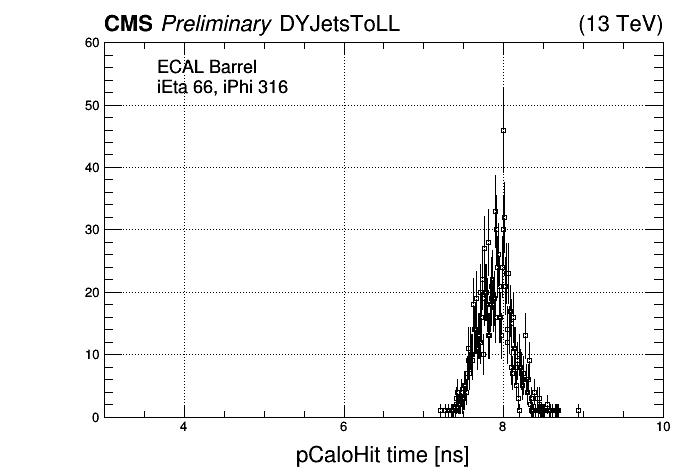
\includegraphics{fig/sec_gen/tr_pcaloMtime0_hist_23112020160113.png}}
\resizebox{0.24\textwidth}{!}{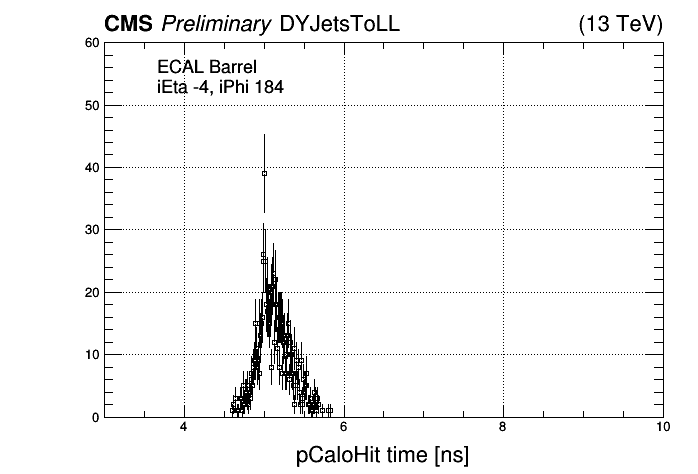
\includegraphics{fig/sec_gen/tr_pcaloMtime1_hist_23112020160311.png}}
\resizebox{0.24\textwidth}{!}{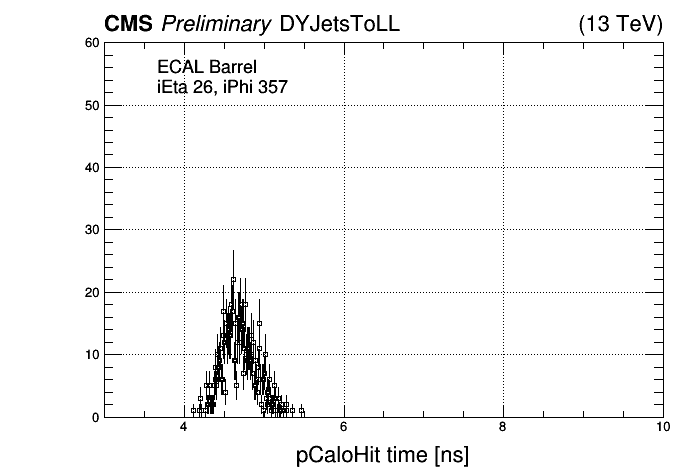
\includegraphics{fig/sec_gen/tr_pcaloMtime2_hist_23112020160510.png}}
\resizebox{0.24\textwidth}{!}{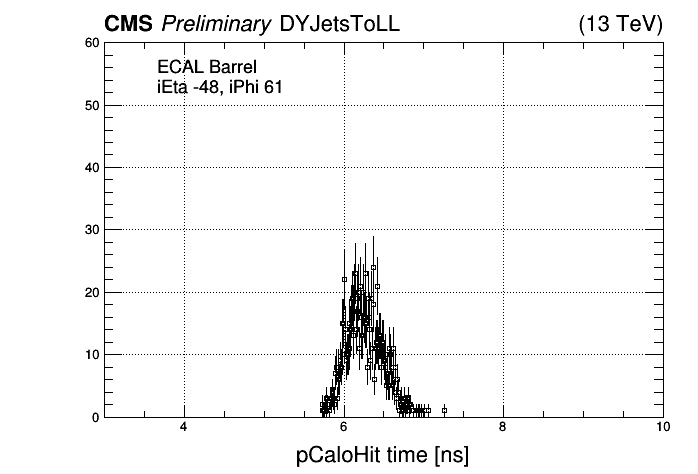
\includegraphics{fig/sec_gen/tr_pcaloMtime3_hist_23112020160828.png}}
\label{pc_4c_pct}}

\subfloat[pCaloHit multiplicity in the four separate crystals studied. ]{
\resizebox{0.24\textwidth}{!}{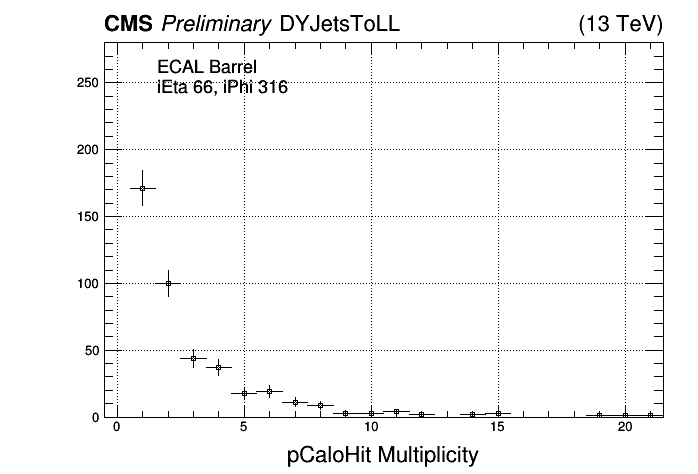
\includegraphics{fig/sec_gen/tr_pcaloMulti0_hist_23112020164218.png}}
\resizebox{0.24\textwidth}{!}{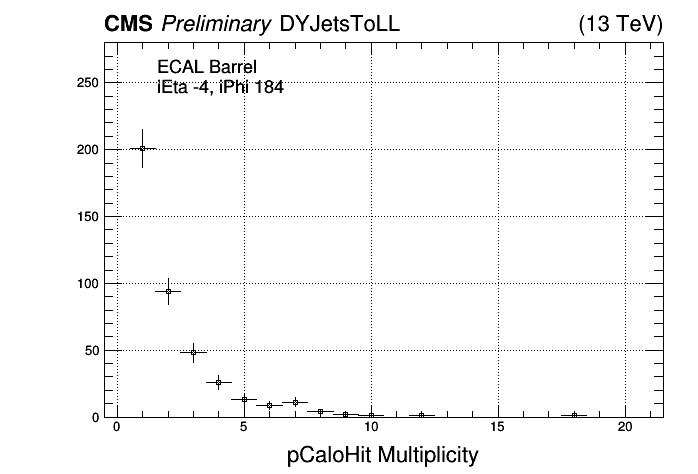
\includegraphics{fig/sec_gen/tr_pcaloMulti1_hist_23112020164317.png}}
\resizebox{0.24\textwidth}{!}{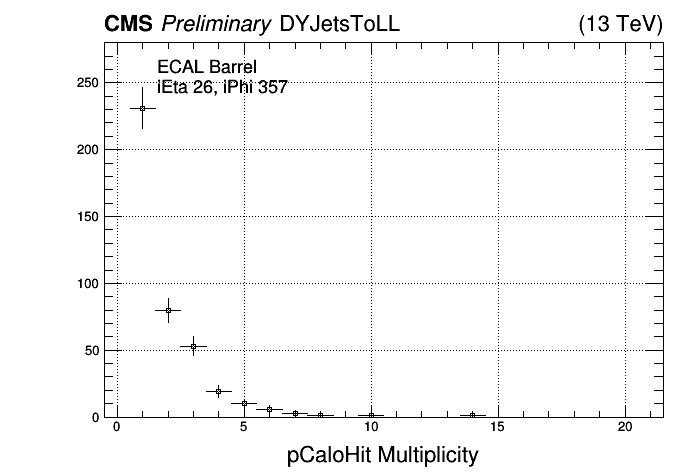
\includegraphics{fig/sec_gen/tr_pcaloMulti2_hist_23112020164503.png}}
\resizebox{0.24\textwidth}{!}{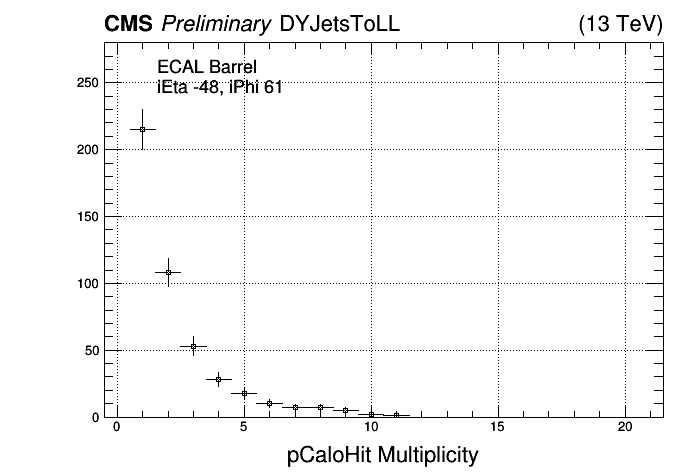
\includegraphics{fig/sec_gen/tr_pcaloMulti3_hist_23112020164600.png}}
%\caption{pCaloHit multiplicity in the four separate crystals studied. } 
\label{pc_4c_pcm}}

\subfloat[Weighted RMS of pCaloHit time in the four separate crystals studied. ]{
\resizebox{0.24\textwidth}{!}{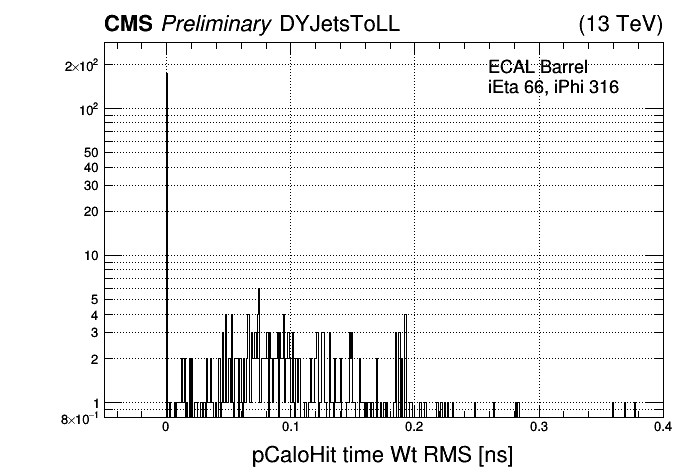
\includegraphics{fig/sec_gen/tr_pcaloWtRMS0_hist_23112020165226.png}}
\resizebox{0.24\textwidth}{!}{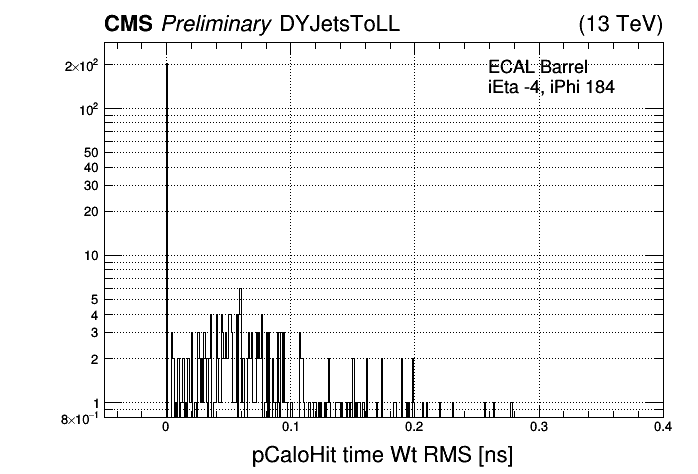
\includegraphics{fig/sec_gen/tr_pcaloWtRMS1_hist_23112020165419.png}}
\resizebox{0.24\textwidth}{!}{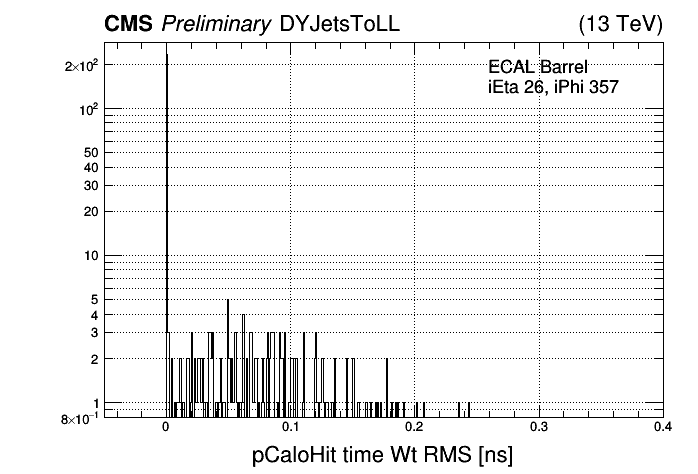
\includegraphics{fig/sec_gen/tr_pcaloWtRMS2_hist_23112020165539.png}}
\resizebox{0.24\textwidth}{!}{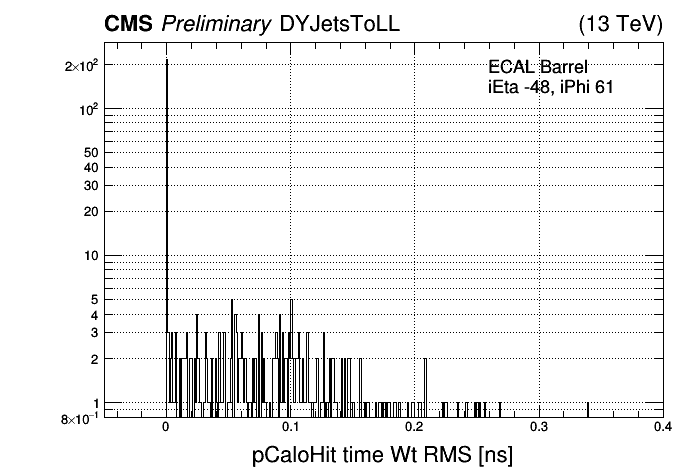
\includegraphics{fig/sec_gen/tr_pcaloWtRMS3_hist_23112020165750.png}}
\label{pc_4c_rms}}
\caption{pCaloHit time distribution, multiplicity, and Wt. RMS of the time for pCaloHits geometrically matched to four separate crystals in ECAL Barrel. These crystals are located, from left to right, at (ieta, iphi) of : (66,316), (26,357), (-4,184), and (-48,61) in the EB. Note that in the Wt. RMS plots the spike at zero correspond to crystal with a single pCaloHit.}
\label{pc_4c_all}
\end{center}
\end{figure} 

These collections of pCaloHits geometrically matched to a single crystal were studied in four randomly selected crystals spread along the ECAL barrel in eta and phi. From the matched pCaloHits in these crystals the energy weighted RMS of the pCaloHit times was determined. In Figure~\ref{pc_4c_all} of the pCaloHit times, multiplicity, and the Wt. RMS of the times in these four crystals are shown. It can be seen that while the mean value the time distributions varies according to the time of flight distance for each of the specific crystals, the distribution of these values are roughly the same in all four crystals with a spread in the times under one nanosecond. In Figure~\ref{pc_rms} the event by event Wt. RMS for the pCaloHit times in all barrel crystals is shown. It can be seen that the Wt. RMS of the pCaloHits, in crystals with a multiplicity greater than one, peaks at $\sim$60-80 ps.

\begin{figure}[htbp]
\begin{center}
%\resizebox{0.48\textwidth}{!}{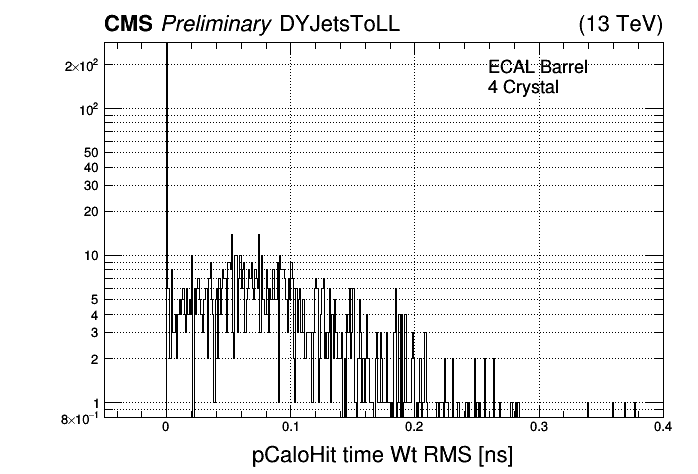
\includegraphics{fig/sec_gen/tr_pcaloWtRMS_hist_23112020165948.png}}
\resizebox{0.7\textwidth}{!}{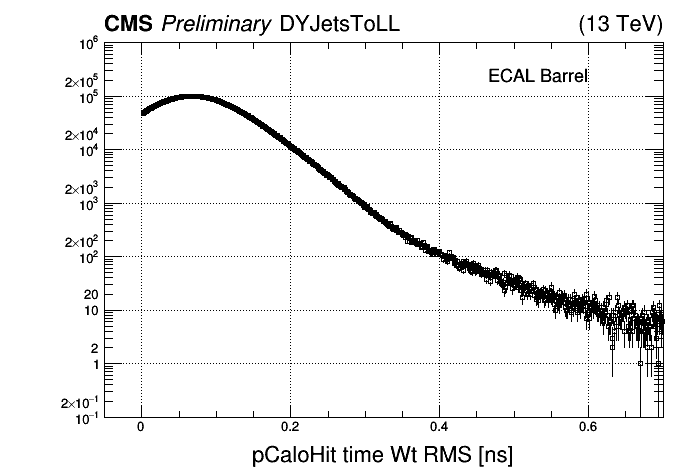
\includegraphics{fig/sec_gen/tr_pcaloWtRMS_hist_07012021124909.png}}
\caption{The event by event Wt. RMS for the pCaloHit times geometrically matched to individual crystals for all crystal in EB. In crystals with a multiplicity greater than one, the Wt. RMS is shown to peak at $\sim$60-80 ps.}
\label{pc_rms}
\end{center}
\end{figure}

The correlations between the sum of the pCaloHit energies, the multiplicity, and the Wt.RMS, as shown in Figure~\ref{pc_sevm}, within the pCaloHits geometrically matched to a crystal were studied. As can be seen in the plot on the top left in Figure~\ref{pc_sevm}, the crystals with larger sums of pCaloHit energies correspond to those with higher multiplicities, as would be expected in terms of shower development. In the top right plot we can see that there is no strong apparent correlation between the sum of the pCaloHit energies in a crystal and the Wt. RMS of the pCaloHit times in that crystal. In the plot on the bottom it can be seen that the Wt. RMS of the pCaloHit times have characteristic range of approximately 80-100 ps that is persistent with increasing multiplicity.

\begin{figure}[htbp]
\begin{center}
%\resizebox{0.48\textwidth}{!}{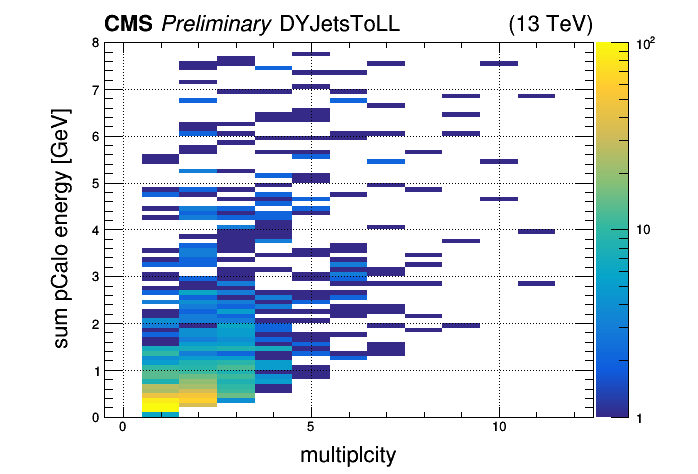
\includegraphics{fig/sec_gen/tr_2d_multi_v_sume_12112020155403.png}}
\resizebox{0.475\textwidth}{!}{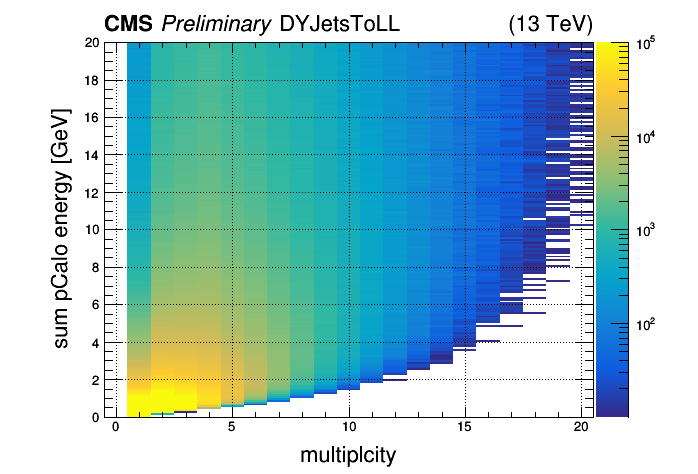
\includegraphics{fig/sec_gen/tr_2d_spcevmulti_07012021143040.png}}
\resizebox{0.475\textwidth}{!}{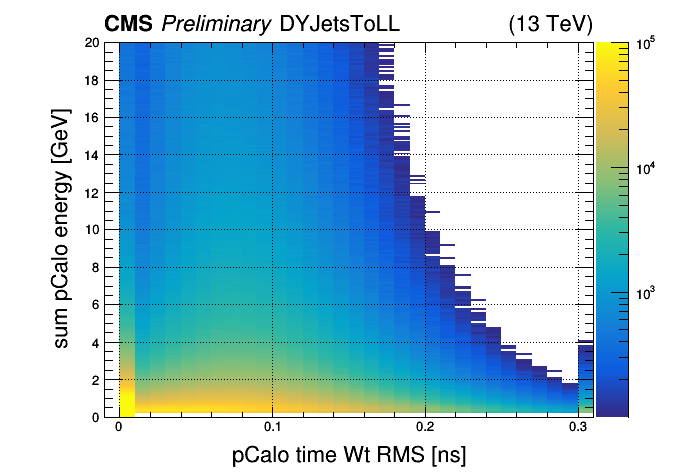
\includegraphics{fig/sec_gen/tr_2d_pcrmsvspce_07012021142215.png}}
\resizebox{0.475\textwidth}{!}{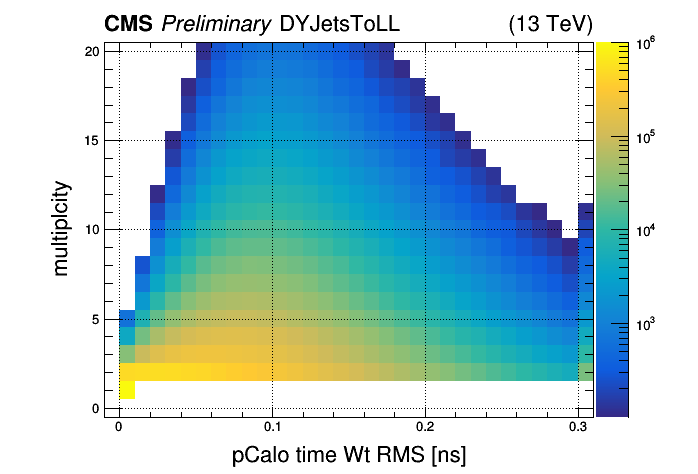
\includegraphics{fig/sec_gen/tr_2d_pcrmsvmulti_07012021142611.png}}
\caption{The correlations between the sum of the pCaloHit energy and the multiplicity (top left), the  Wt. RMS of the pCaloHit times and the sum of the pCaloHit energy (top right), and the Wt. RMS of the pCaloHit times and the pCaloHit multiplicity (bottom) for pCaloHits geometrically matched to a crystal. }
\label{pc_sevm}
\end{center}
\end{figure}

%\begin{figure}[htbp]
%\begin{center}
%\resizebox{0.48\textwidth}{!}{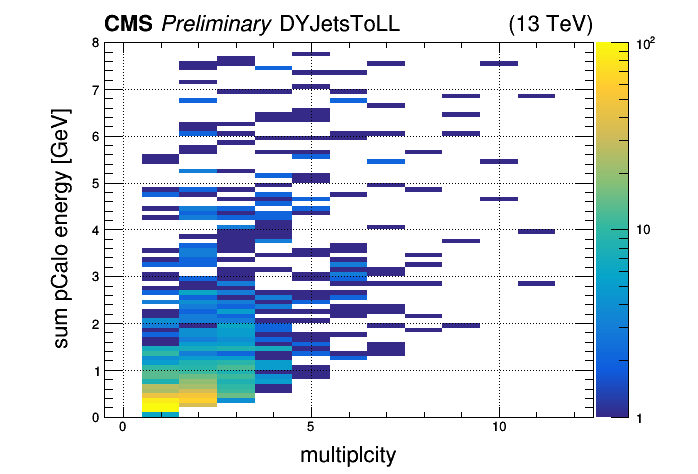
\includegraphics{fig/sec_gen/tr_2d_multi_v_sume_12112020155403.png}}
%\resizebox{0.48\textwidth}{!}{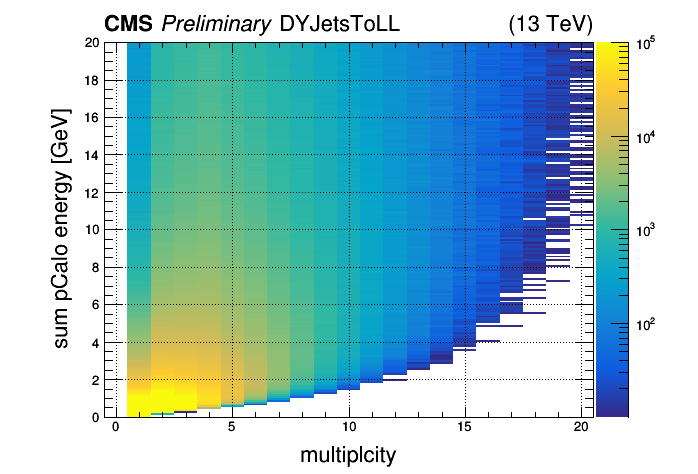
\includegraphics{fig/sec_gen/tr_2d_spcevmulti_07012021143040.png}}
%\caption{Sum pCaloHit energy correlated to pCaloHit multiplicity. }
%\label{pc_sevm}
%\end{center}
%\end{figure}

%\begin{figure}[htbp]
%\begin{center}
%\resizebox{0.48\textwidth}{!}{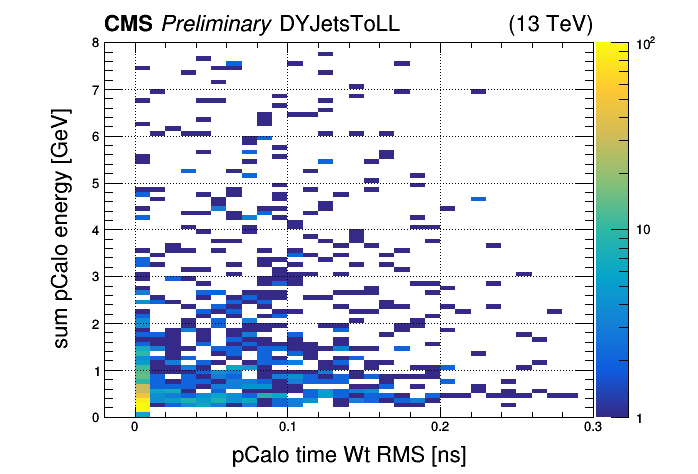
\includegraphics{fig/sec_gen/tr_2d_wtrms_v_sume_12112020155004.png}}
%\resizebox{0.48\textwidth}{!}{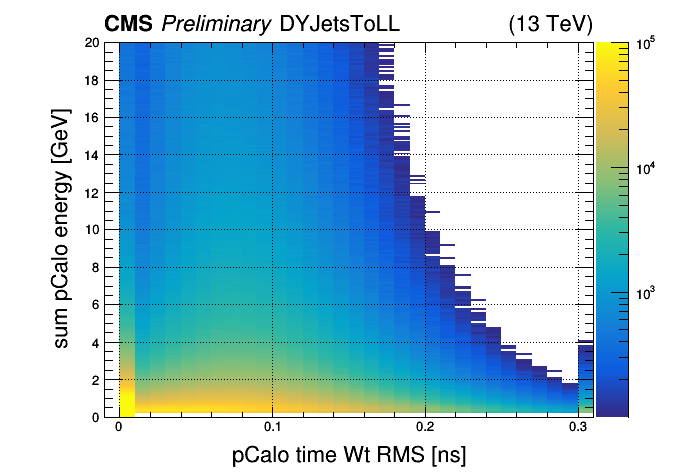
\includegraphics{fig/sec_gen/tr_2d_pcrmsvspce_07012021142215.png}}
%\caption{Sum pCaloHit energy correlated to pCaloHit time weighted RMS. }
%\label{pc_sevrms}
%\end{center}
%\end{figure}

%\begin{figure}[htbp]
%\begin{center}
%\resizebox{0.48\textwidth}{!}{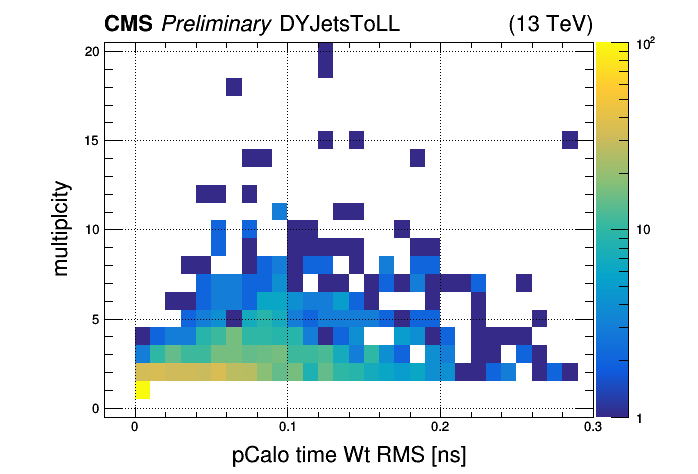
\includegraphics{fig/sec_gen/tr_2d_wtrms_v_multi_12112020154432.png}}
%\resizebox{0.48\textwidth}{!}{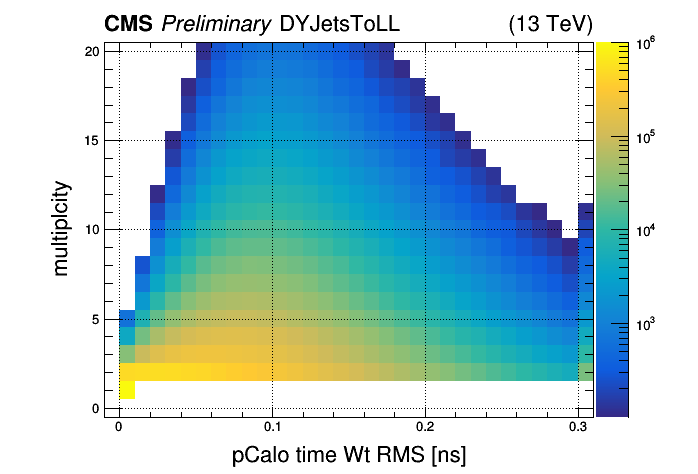
\includegraphics{fig/sec_gen/tr_2d_pcrmsvmulti_07012021142611.png}}
%\caption{pCaloHit multiplicity correlated to pCaloHit time weighted RMS. }
%\label{pc_mvrms}
%\end{center}
%\end{figure}

The gen time for a rechit is calculated as the energy weighted average of the pCaloHit times that have an pCaloHit energy of at least 100 MeV for all pCaloHits geometrically matched to the crystal the rechit was in, as shown in Equation~\ref{eq_gentime}.

\begin{equation} 
\emph{Gen Time} = \frac{\sum( pCaloHit time * pCaloHit energy )}{\sum pCaloHit energy }
\label{eq_gentime}
\end{equation}

The distribution of the gen times in the same four crystals that were previously referenced are shown in Figure~\ref{pc_4c_wat}. Since the actual values recorded for the pCaloHit times are the time since the bunch crossing at CMS origin at which an interacting particle deposited the energy if the pCaloHit in a particular crystal, the pCAloHit times in the EB are expected to vary from $\sim$4-12 ns. The distribution of the weighted average pCaloHit times seen in Figure~\ref{pc_4c_wat} are consistent with the expected mean time given the geometrical location of the selected crystals. In Figure~\ref{pc_wat} the gen times for all EB crystal where the corresponding rechit energy is between 10 GeV and 120 GeV is shown. Consistent with the distributions seen in Figure~\ref{pc_4c_wat} for a single crystal, the time distribution spreads between five and ten nanoseconds as expected, given the time of flight from the CMS origin to the physical location of the crystals.

\hfill
\begin{figure}[htbp]
\begin{center}
\resizebox{0.45\textwidth}{!}{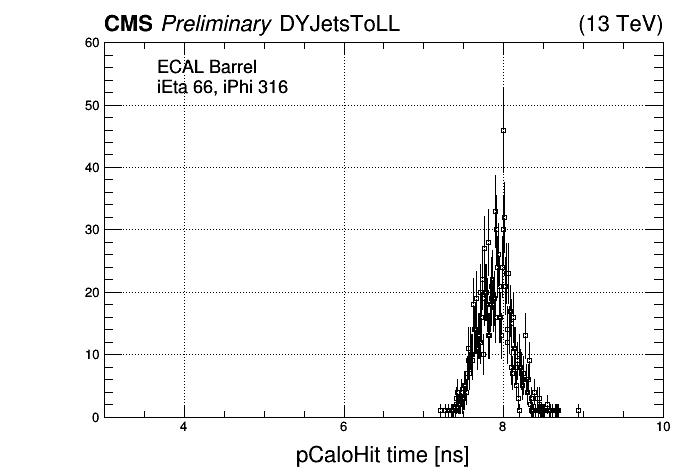
\includegraphics{fig/sec_gen/tr_pcaloMtime0_hist_23112020160113.png}}
\resizebox{0.45\textwidth}{!}{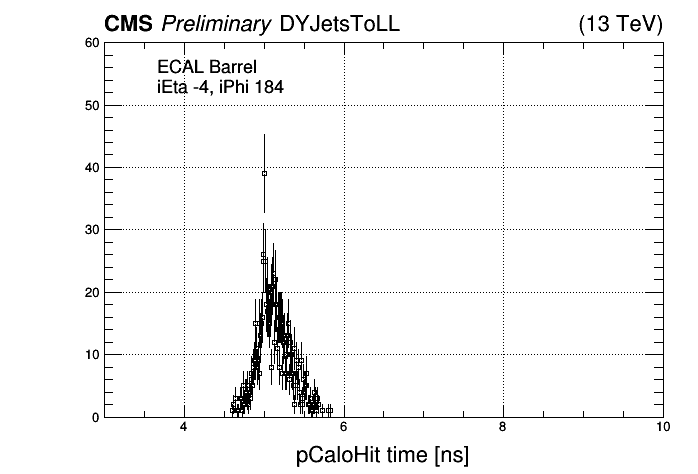
\includegraphics{fig/sec_gen/tr_pcaloMtime1_hist_23112020160311.png}}
\resizebox{0.45\textwidth}{!}{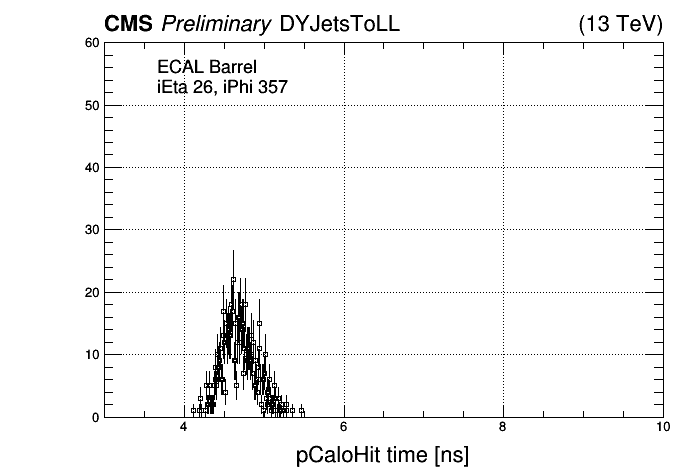
\includegraphics{fig/sec_gen/tr_pcaloMtime2_hist_23112020160510.png}}
\resizebox{0.45\textwidth}{!}{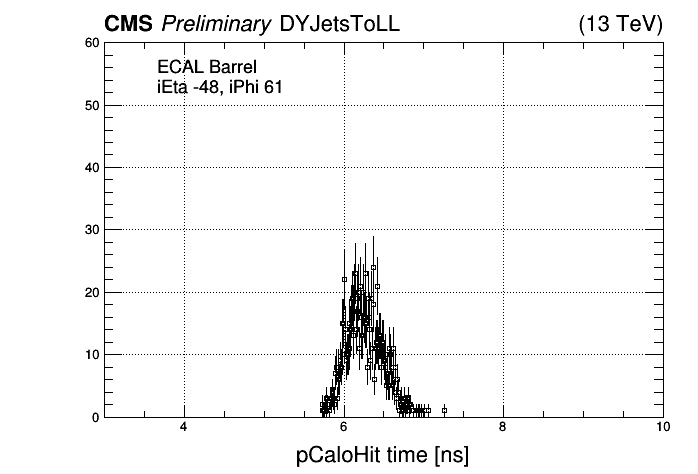
\includegraphics{fig/sec_gen/tr_pcaloMtime3_hist_23112020160828.png}}
\caption{Weighted average pCaloHit time, or gen time, in the four separate crystal of the pCalo hits geometrically matched to those crystals. These crystals are located, in order left to right, top to bottom, at (ieta, iphi) of : (66,316), (26,357), (-4,184), and (-48,61) in the EB.} 
\label{pc_4c_wat}
\end{center}
\end{figure} 

%\begin{figure}[htbp]
%\begin{center}
%\resizebox{0.42\textwidth}{!}{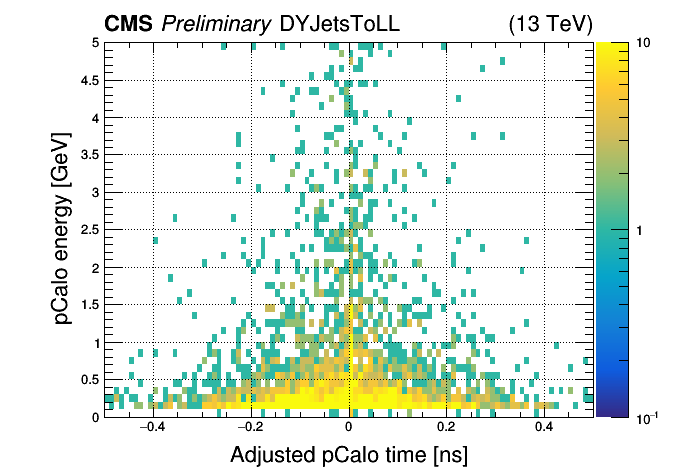
\includegraphics{fig/sec_gen/tr_2d_pctve_24112020141604.png}}
%\resizebox{0.42\textwidth}{!}{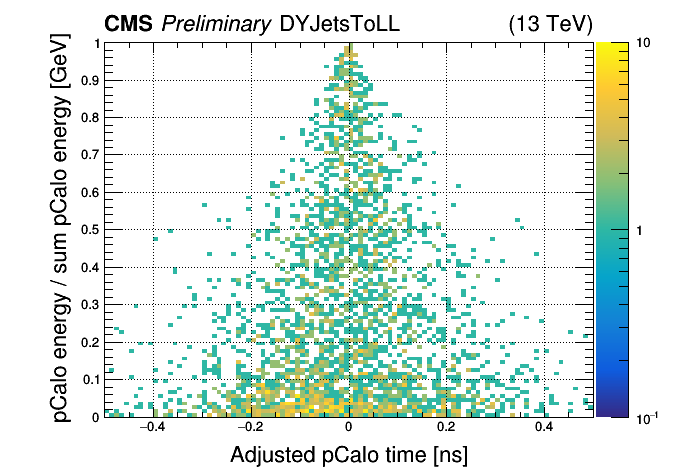
\includegraphics{fig/sec_gen/tr_2d_pctvne_24112020141913.png}}
%\resizebox{0.42\textwidth}{!}{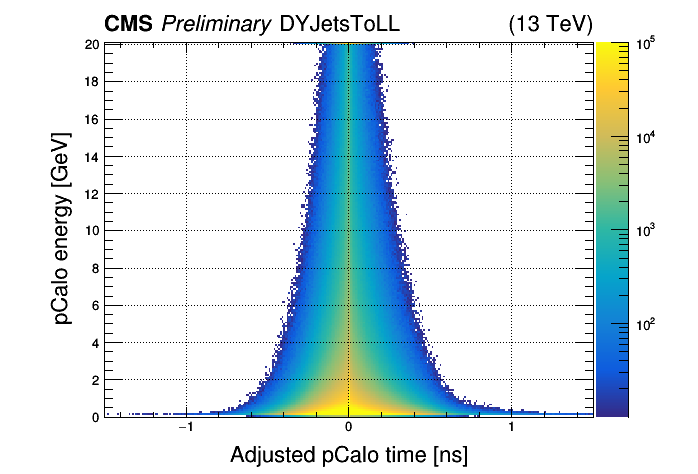
\includegraphics{fig/sec_gen/tr_2d_apctvpce_07012021145909.png}}
%\resizebox{0.42\textwidth}{!}{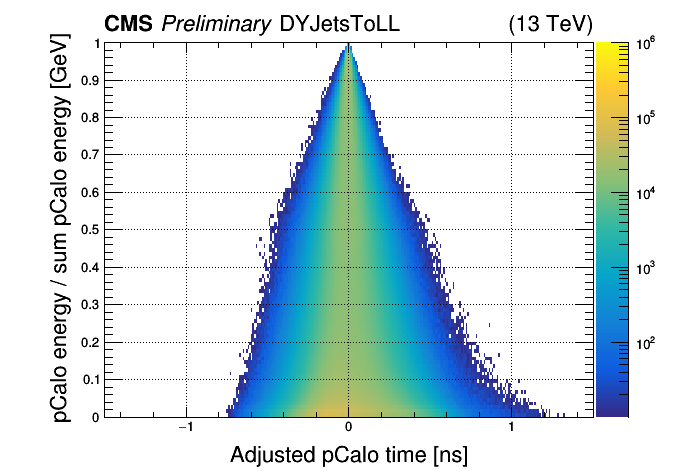
\includegraphics{fig/sec_gen/tr_2d_apctvnpce_07012021150111.png}}
%\caption{Adjusted pCaloHit time [ns] with respect to pCalo energy [GeV]. The pCalo time is adjusted by subtracting the weighted average time of the pCalo hits from the time of the individual pCalo hits. In the right hand plot the pCalo energy is normalized by the sum of the pCalo energies.}
%\label{pc_adjtve}
%\end{center}
%\end{figure} 

%\begin{figure}[htbp]
%\begin{center}
%\resizebox{0.42\textwidth}{!}{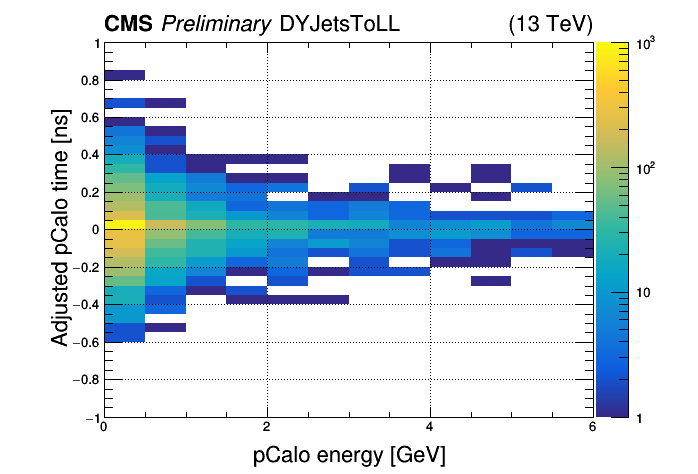
\includegraphics{fig/sec_gen/tr_pcalo_calitve_hist_17112020185058.png}}
%\resizebox{0.42\textwidth}{!}{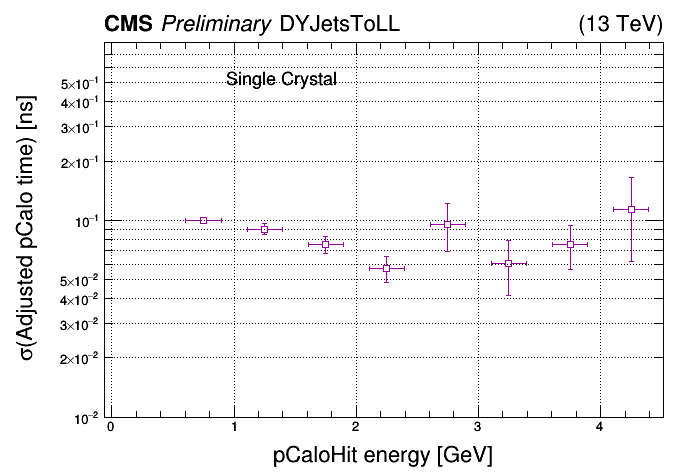
\includegraphics{fig/sec_gen/tr_mc_sp_plot_17112020185336.png}}
%\resizebox{0.42\textwidth}{!}{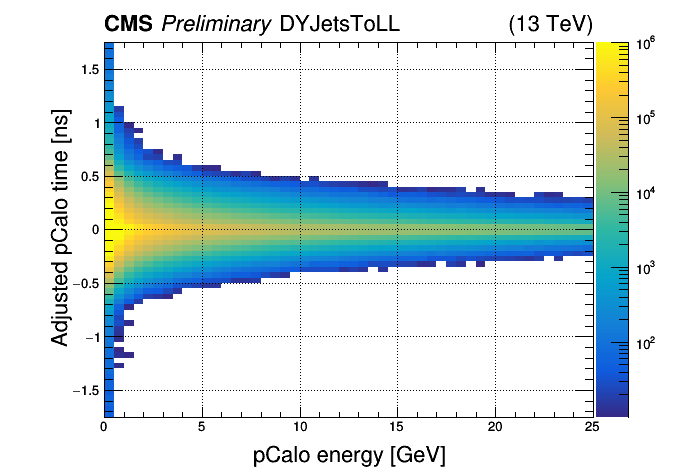
\includegraphics{fig/sec_gen/tr_2d_mcDataHist_13012021134816.png}}
%\resizebox{0.42\textwidth}{!}{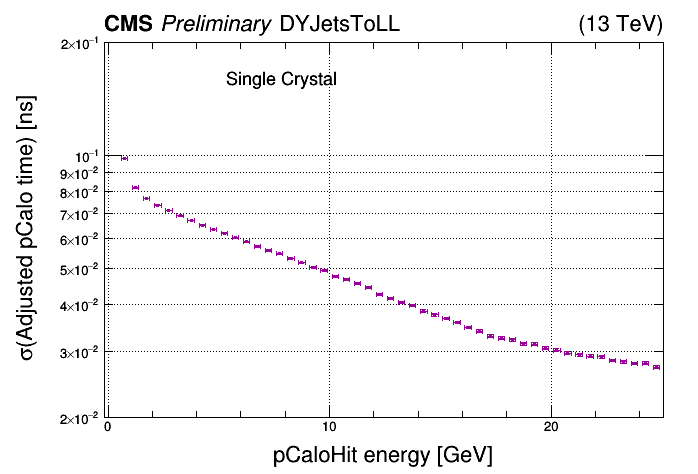
\includegraphics{fig/sec_gen/tr_mc_sp_plot_19012021181820.png}}
%\caption{Single crystal time distribution widths of adjusted pCalo times [ns] with respect to pCalo energy [GeV].}
%\label{pc_pctve_scres}
%\end{center}
%\end{figure} 

The times reconstructed by the timing algorithms, once calibrated, are shifted so that the average time of all hits in a particular crystal is zero. This effectively shifts the mean time of a rechit in each crystal to be zero with respect to the time that the bunch crossing theoretically occurs at the CMS origin. In order to compare the pCalo gen times to the rechit times it is necessary to shift the gen times so that the gen time and the rechit time are both in the same temporal frame of reference. The gen times include the difference in time between the theoretical BX time at the origin and the time that an interaction occurred in the crystal, as well as the the flight time for a particle from the interaction vertex to the physical location of the crystals. To account for the difference between the actual interaction vertex for an event and the rechit time in a global resolution study, the rechit times are TOF corrected from the CMS origin to the physical location of the crystal in which the rechit occurs and are then TOF shifted from the crystal location to the location of the PV. This effectively regresses the time of the rechit back to the time when the particle that produced the rechit was created. To bring the gen times into the same temporal frame of reference they are TOF shifted from the physical crystal location to the position of the PV, therefore also shifting the gen time from the time of the particle interaction with the crystal to the time that the particle which interacted with the crystal was theoretically produced in the PV. In the case of a local resolution study, the TOF correction are also made to the rechit times but have a negligible impact on the local resolution.

\begin{figure}[htbp]
\begin{center}
\resizebox{0.7\textwidth}{!}{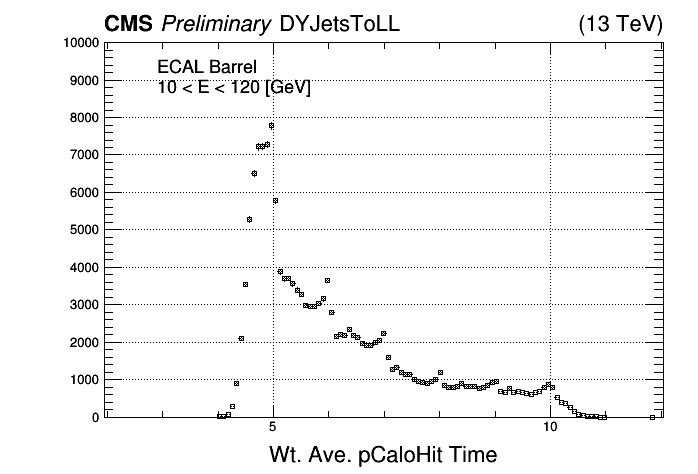
\includegraphics{fig/sec_gen/tr_pcalo_raw_wt_ave_time_hist_15122020161151.png}}
\caption{Gen time for rechits with energies between 10 GeV and 120 GeV in the EB. The gen time distribution is spread between $\sim$4-12 ns, as is to be expected given the time of flight from the CMS origin to the physical location of the crystals.}
\label{pc_wat}
\end{center}
\end{figure}

Using the gen time obtained from the TOF adjusted average weighted pCalo time as a truth time has several limitations. As mentioned previously, the depth of the energy deposition recorded by the pCalo hits does not preserve the information of the depth of deposition in the crystal. The pCalo hits do not reflect the variations arising from the location of the hit on the crystal face or the light collection efficiency of the crystal, and the TOF adjustments are sensitive to the resolution of the primary vertex. These limiting factors mean that it is not possible to archive a perfect resolution with this method of producing a truth time. As can be seen in Figure~\ref{pc_scres}, though, approximately the same resolution is achieved across all energies, for both the Same RO unit and the $Z\rightarrow e^{+}e^{-}$ cases, of $\sim$80-90 ps.

\begin{figure}[htbp]
\begin{center}
\resizebox{0.7\textwidth}{!}{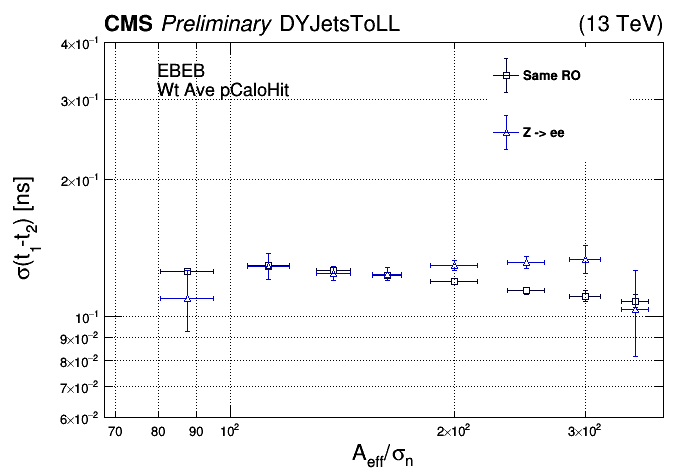
\includegraphics{fig/sec_gen/tr_mc_lgres_plot_15112021155242.png}}
\caption{Same RO and $Z\rightarrow e^{+}e^{-}$ resolutions in DYjetsToLL MC for pCAlo gen time. Roughly the same resolution of $\sim$80-90 ps is achieved across all energies for both the Same RO unit and the $Z\rightarrow e^{+}e^{-}$ cases.} 
\label{pc_scres}
\end{center}
\end{figure} 

Since the data used as input for the timing reconstruction methods is derived from the pCaloHit collection, the resolution obtained using the pCaloHit gen time reference is the best resolution achievable by the timing reconstruction with a particular MC data stream. 


%********* intros PV resolution and crystal face hit location approximation effects to gen time resolutions ... 
% ... only explain our method of obtaining a gen time then -> see below .....
%.... make statements about limitations in current gen times from pcalo from most recent gen time studies talk in ecal moca meeting Apr 28 2021 ....
%... end section with pcalo vs cc \& ratio single crystal resolutions in MC ......




%\begin{figure}[htbp]
%\begin{center}
%\resizebox{0.22\textwidth}{!}{\includegraphics{fig/sec_gen/tr_pcalo}}
%\resizebox{0.22\textwidth}{!}{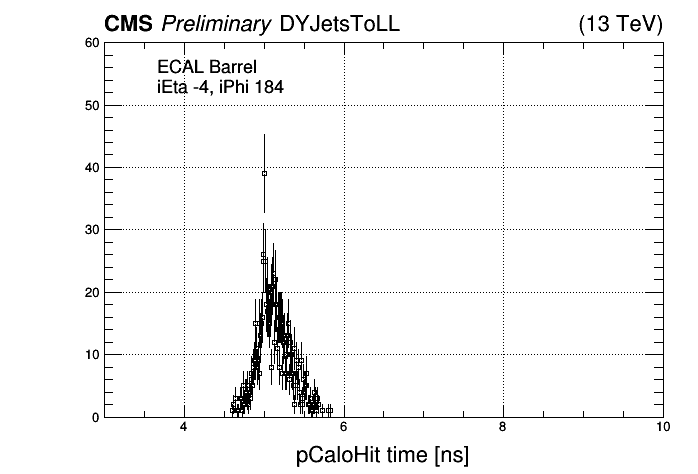
\includegraphics{fig/sec_gen/tr_pcaloMtime1_hist_23112020160311.png}}
%\resizebox{0.22\textwidth}{!}{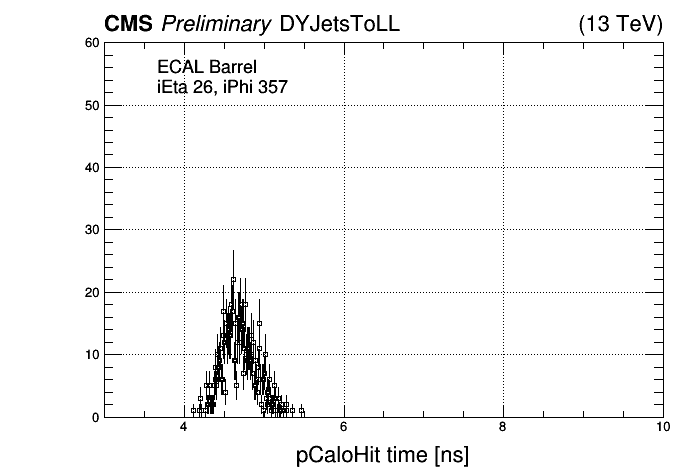
\includegraphics{fig/sec_gen/tr_pcaloMtime2_hist_23112020160510.png}}
%\resizebox{0.22\textwidth}{!}{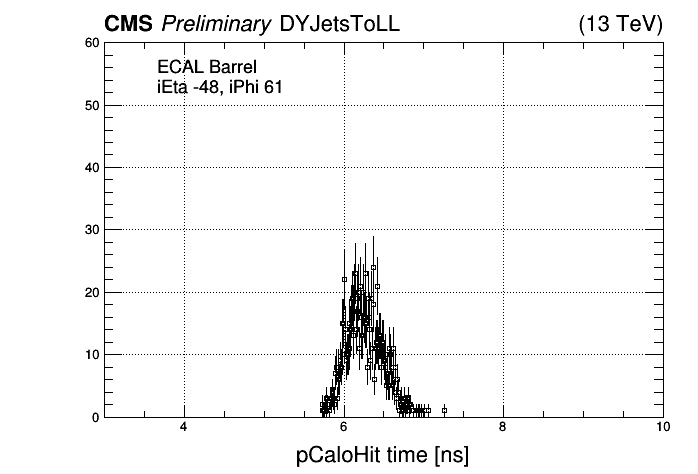
\includegraphics{fig/sec_gen/tr_pcaloMtime3_hist_23112020160828.png}}
%\caption{pCaloHit energy in the four separate crystals studied. } 
%\label{pc_4c_pce}
%\end{center}
%\end{figure} 

